\documentclass[10pt]{beamer}
\usetheme{Madrid}
\usecolortheme{seahorse}
\usepackage[utf8]{inputenc}
\usepackage[T1]{fontenc}
\usepackage{listings}
\usepackage{tikz}
\usepackage{booktabs}
\usepackage{amssymb}
\usepackage{amsmath}
\usetikzlibrary{arrows.meta,positioning,shapes.geometric,fit,calc}
\definecolor{jugeoBlue}{RGB}{25,84,166}
\definecolor{jugeoDark}{RGB}{15,50,100}
\definecolor{jugeoLight}{RGB}{200,220,255}
\definecolor{jugeoGreen}{RGB}{0,128,60}
\definecolor{jugeoRed}{RGB}{180,30,30}
\definecolor{jugeoOrange}{RGB}{210,120,20}
\newcommand{\jugmark}[1]{\textcolor{jugeoBlue}{\textbf{#1}}}
\lstset{
  language=Python,
  basicstyle=\ttfamily\scriptsize,
  keywordstyle=\color{jugeoBlue}\bfseries,
  stringstyle=\color{jugeoGreen},
  commentstyle=\color{gray}\itshape,
  backgroundcolor=\color{jugeoLight!30},
  frame=single,
  framerule=0.5pt,
  rulecolor=\color{jugeoBlue!50},
  breaklines=true,
  showstringspaces=false,
  tabsize=2,
  columns=flexible
}
\begin{document}
% Part VIII — Vision, Comparison, and Wrap-Up (Slides 181–200)
\providecommand{\jugmark}[1]{\textbf{\color{jugeoBlue}#1}}

% ---------------------------------------------------------------------------
% Slide 181: Section divider — Part VIII
% ---------------------------------------------------------------------------
\begin{frame}
\frametitle{}
\vfill
\begin{center}
  {\Huge\color{jugeoBlue}\textbf{Part VIII}}\\[12pt]
  {\LARGE\color{jugeoDark}The Big Picture}\\[20pt]
  
\begin{tikzpicture}
    \draw[jugeoBlue, line width=2pt] (-3,0) -- (3,0);
  \end{tikzpicture}\\[12pt]
  {\large\color{gray}\itshape Vision, comparison, and where we go from here}
\end{center}
\vfill
\end{frame}

% ---------------------------------------------------------------------------
% Slide 182: The Four Bets
% ---------------------------------------------------------------------------
\begin{frame}
\frametitle{The Four Bets}
JuGeo stakes its design on \jugmark{four fundamental bets}:
\vspace{8pt}
\begin{center}
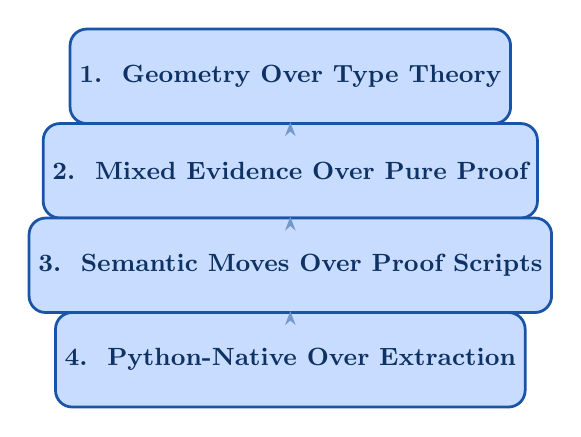
\begin{tikzpicture}[
    bet/.style={rectangle, rounded corners=6pt, draw=jugeoBlue, fill=jugeoLight,
                minimum width=52mm, minimum height=12mm, font=\small\bfseries,
                line width=1pt, text=jugeoDark},
    arr/.style={-{Stealth[length=5pt]}, jugeoBlue!60, line width=0.8pt}
  ]
  \node[bet] (b1) at (0, 2.4) {1.\ \ Geometry Over Type Theory};
  \node[bet] (b2) at (0, 1.2) {2.\ \ Mixed Evidence Over Pure Proof};
  \node[bet] (b3) at (0, 0.0) {3.\ \ Semantic Moves Over Proof Scripts};
  \node[bet] (b4) at (0,-1.2) {4.\ \ Python-Native Over Extraction};
  \draw[arr] (b1)--(b2);
  \draw[arr] (b2)--(b3);
  \draw[arr] (b3)--(b4);
\end{tikzpicture}
\end{center}
\vspace{6pt}
\begin{center}
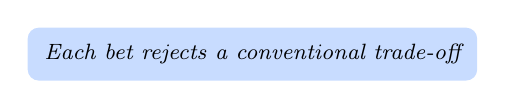
\begin{tikzpicture}
  \node[fill=jugeoLight, rounded corners, inner sep=6pt, font=\footnotesize\itshape]
    {Each bet rejects a conventional trade-off};
\end{tikzpicture}
\end{center}
\end{frame}

% ---------------------------------------------------------------------------
% Slide 183: Bet 1 — Geometry Over Type Theory
% ---------------------------------------------------------------------------
\begin{frame}
\frametitle{Bet 1 --- Geometry Over Type Theory}
\begin{columns}[T]
\begin{column}{0.48\textwidth}
\begin{alertblock}{Conventional}
  \begin{itemize}
    \item Proofs are \textbf{terms}
    \item Type-check: pass / fail
    \item Failure = opaque error
  \end{itemize}
\end{alertblock}
\end{column}
\begin{column}{0.48\textwidth}
\begin{exampleblock}{JuGeo}
  \begin{itemize}
    \item Proofs are \jugmark{sections over sites}
    \item Local claims glue globally
    \item Failure = structured obstruction
  \end{itemize}
\end{exampleblock}
\end{column}
\end{columns}
\vspace{10pt}
\begin{center}
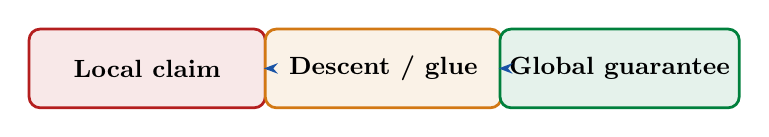
\begin{tikzpicture}[
    box/.style={rectangle, rounded corners=4pt,
                minimum width=30mm, minimum height=10mm, font=\small\bfseries,
                line width=1pt}
  ]
  \node[box, draw=jugeoRed, fill=jugeoRed!10]     (local) at (-3,0) {Local claim};
  \node[box, draw=jugeoOrange, fill=jugeoOrange!10] (glue)  at ( 0,0) {Descent / glue};
  \node[box, draw=jugeoGreen, fill=jugeoGreen!10]  (glob)  at ( 3,0) {Global guarantee};
  \draw[-{Stealth[length=5pt]}, line width=1pt, jugeoBlue] (local)--(glue);
  \draw[-{Stealth[length=5pt]}, line width=1pt, jugeoBlue] (glue)--(glob);
\end{tikzpicture}
\end{center}
\end{frame}

% ---------------------------------------------------------------------------
% Slide 184: Bet 2 — Mixed Evidence Over Pure Proof
% ---------------------------------------------------------------------------
\begin{frame}
\frametitle{Bet 2 --- Mixed Evidence Over Pure Proof}
\begin{block}{The Problem with Binary}
  Traditional systems: either you have a \textbf{proof} or you have \textbf{nothing}.\\[4pt]
  Real projects have partial evidence everywhere.
\end{block}
\vspace{6pt}
\begin{center}
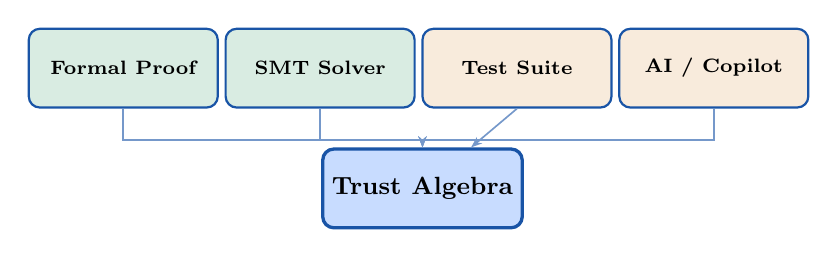
\begin{tikzpicture}[
    ch/.style={rectangle, rounded corners=4pt, draw=jugeoBlue,
               minimum width=24mm, minimum height=10mm, font=\scriptsize\bfseries,
               line width=0.8pt},
    arr/.style={-{Stealth[length=4pt]}, jugeoBlue!60, line width=0.6pt}
  ]
  \node[ch, fill=jugeoGreen!15]  (proof) at (-4, 0) {Formal Proof};
  \node[ch, fill=jugeoGreen!15]  (smt)   at (-1.5,0) {SMT Solver};
  \node[ch, fill=jugeoOrange!15] (test)  at ( 1, 0) {Test Suite};
  \node[ch, fill=jugeoOrange!15] (ai)    at ( 3.5,0) {AI / Copilot};

  \node[rectangle, rounded corners=4pt, draw=jugeoBlue, fill=jugeoLight,
        minimum width=18mm, minimum height=10mm, font=\small\bfseries,
        line width=1.2pt, below=14pt of test, xshift=-12mm] (trust) {Trust Algebra};

  \draw[arr] (proof.south) -- ++(0,-0.4) -| (trust);
  \draw[arr] (smt.south)   -- ++(0,-0.4) -| (trust);
  \draw[arr] (test.south)  -- (trust);
  \draw[arr] (ai.south)    -- ++(0,-0.4) -| (trust);
\end{tikzpicture}
\end{center}
\vspace{4pt}
\begin{center}
  {\small JuGeo's \jugmark{trust algebra} combines all channels honestly --- no pretending.}
\end{center}
\end{frame}

% ---------------------------------------------------------------------------
% Slide 185: Bet 3 — Semantic Moves Over Proof Scripts
% ---------------------------------------------------------------------------
\begin{frame}
\frametitle{Bet 3 --- Semantic Moves Over Proof Scripts}
\begin{columns}[T]
\begin{column}{0.48\textwidth}
\begin{alertblock}{Proof Scripts}
  \begin{itemize}
    \item \texttt{apply}, \texttt{rewrite}, \texttt{simp}
    \item Syntax-level manipulation
    \item User picks every tactic
  \end{itemize}
\end{alertblock}
\end{column}
\begin{column}{0.48\textwidth}
\begin{exampleblock}{JuGeo Tactics}
  \begin{itemize}
    \item Operate on \jugmark{proof geometry}
    \item Coordinates, covers, trust, obstructions
    \item \jugmark{Adaptive control} selects tactics
  \end{itemize}
\end{exampleblock}
\end{column}
\end{columns}
\vspace{10pt}
\begin{center}
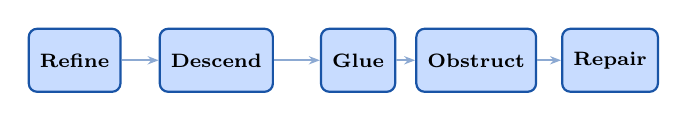
\begin{tikzpicture}[
    mv/.style={rectangle, rounded corners=3pt, draw=jugeoBlue, fill=jugeoLight,
               minimum height=8mm, font=\scriptsize\bfseries, line width=0.8pt,
               inner xsep=4pt}
  ]
  \node[mv] (r) at (-3.6,0) {Refine};
  \node[mv] (d) at (-1.8,0) {Descend};
  \node[mv] (g) at ( 0,0)   {Glue};
  \node[mv] (o) at ( 1.5,0) {Obstruct};
  \node[mv] (p) at ( 3.2,0) {Repair};
  \foreach \a/\b in {r/d, d/g, g/o, o/p}
    \draw[-{Stealth[length=4pt]}, jugeoBlue!50, line width=0.6pt] (\a)--(\b);
\end{tikzpicture}
\end{center}
{\small Tactics are \jugmark{semantic moves} on a geometric proof state, not syntactic rewrites.}
\end{frame}

% ---------------------------------------------------------------------------
% Slide 186: Bet 4 — Python-Native Over Extraction
% ---------------------------------------------------------------------------
\begin{frame}
\frametitle{Bet 4 --- Python-Native Over Extraction}
\begin{center}
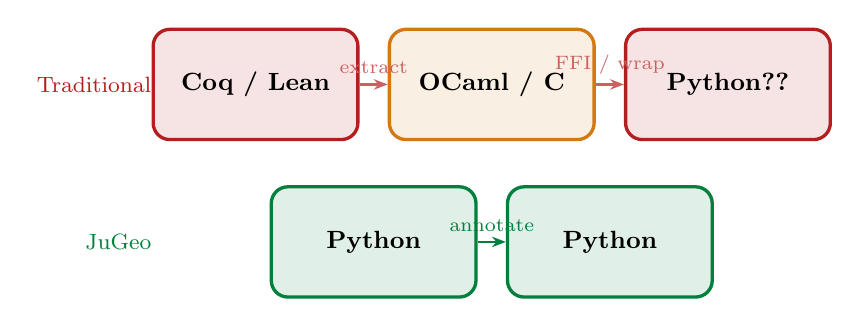
\begin{tikzpicture}[
    lang/.style={rectangle, rounded corners=6pt,
                 minimum width=26mm, minimum height=14mm, font=\small\bfseries,
                 line width=1.2pt},
    arr/.style={-{Stealth[length=5pt]}, line width=1pt}
  ]
  % Traditional path
  \node[lang, draw=jugeoRed, fill=jugeoRed!12]      (coq)  at (-3, 1.2) {Coq / Lean};
  \node[lang, draw=jugeoOrange, fill=jugeoOrange!12] (ocml) at ( 0, 1.2) {OCaml / C};
  \node[lang, draw=jugeoRed, fill=jugeoRed!12]      (py1)  at ( 3, 1.2) {Python??};
  \draw[arr, jugeoRed!70]  (coq)--(ocml) node[midway,above,font=\scriptsize]{extract};
  \draw[arr, jugeoRed!70]  (ocml)--(py1) node[midway,above,font=\scriptsize]{FFI / wrap};

  % JuGeo path
  \node[lang, draw=jugeoGreen, fill=jugeoGreen!12]  (py2)  at (-1.5,-0.8) {Python};
  \node[lang, draw=jugeoGreen, fill=jugeoGreen!12]  (py3)  at ( 1.5,-0.8) {Python};
  \draw[arr, jugeoGreen]   (py2)--(py3) node[midway,above,font=\scriptsize]{annotate};

  % Labels
  \node[font=\footnotesize\color{jugeoRed}, anchor=east]   at (-4.2,1.2) {Traditional};
  \node[font=\footnotesize\color{jugeoGreen}, anchor=east] at (-4.2,-0.8) {JuGeo};
\end{tikzpicture}
\end{center}
\vspace{6pt}
\begin{itemize}
  \item If you \jugmark{ship Python}, the proof should \jugmark{be Python}
  \item Annotated with coordinates and support
  \item Any verifier can reconstruct the argument from the source
\end{itemize}
\end{frame}

% ---------------------------------------------------------------------------
% Slide 187: Comprehensive Comparison — Part 1
% ---------------------------------------------------------------------------
\begin{frame}
\frametitle{Comparison with Existing Systems (1/3)}
\begin{center}
\small
\begin{tabular}{@{} l c c c c @{}}
\toprule
\textbf{Feature} & \textbf{Lean\,4} & \textbf{Coq} & \textbf{F*} & \textbf{JuGeo} \\
\midrule
Dependent types
  & \color{jugeoGreen}\checkmark
  & \color{jugeoGreen}\checkmark
  & \color{jugeoGreen}\checkmark
  & \color{gray}---\\[2pt]
Refinement types
  & \color{gray}---
  & \color{gray}---
  & \color{jugeoGreen}\checkmark
  & \color{jugeoGreen}\checkmark \\[2pt]
Effect system
  & \color{gray}---
  & \color{gray}---
  & \color{jugeoGreen}\checkmark
  & \color{jugeoGreen}\checkmark \\[2pt]
SMT integration
  & \color{gray}limited
  & \color{gray}---
  & \color{jugeoGreen}\checkmark
  & \color{jugeoGreen}\checkmark \\[2pt]
Tactic framework
  & \color{jugeoGreen}\checkmark
  & \color{jugeoGreen}\checkmark
  & \color{gray}limited
  & \color{jugeoGreen}\checkmark \\
\bottomrule
\end{tabular}
\end{center}
\vspace{6pt}
\begin{center}
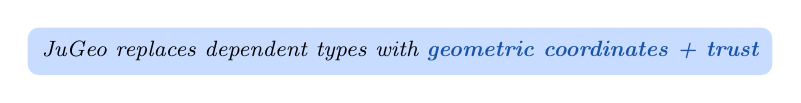
\begin{tikzpicture}
  \node[fill=jugeoLight, rounded corners, inner sep=5pt, font=\footnotesize\itshape]
    {JuGeo replaces dependent types with \jugmark{geometric coordinates + trust}};
\end{tikzpicture}
\end{center}
\end{frame}

% ---------------------------------------------------------------------------
% Slide 188: Comprehensive Comparison — Part 2
% ---------------------------------------------------------------------------
\begin{frame}
\frametitle{Comparison with Existing Systems (2/3)}
\begin{center}
\small
\begin{tabular}{@{} l c c c c @{}}
\toprule
\textbf{Feature} & \textbf{Lean\,4} & \textbf{Coq} & \textbf{F*} & \textbf{JuGeo} \\
\midrule
Code target
  & {\scriptsize C / IR}
  & {\scriptsize OCaml}
  & {\scriptsize C / F\#}
  & \color{jugeoGreen}{\scriptsize Python} \\[2pt]
Trust model
  & {\scriptsize binary}
  & {\scriptsize binary}
  & {\scriptsize binary}
  & \color{jugeoGreen}{\scriptsize 7 levels} \\[2pt]
Evidence channels
  & {\scriptsize 1}
  & {\scriptsize 1}
  & {\scriptsize 2}
  & \color{jugeoGreen}{\scriptsize 4+} \\[2pt]
Failure model
  & {\scriptsize error msg}
  & {\scriptsize error msg}
  & {\scriptsize error msg}
  & \color{jugeoGreen}{\scriptsize obstruction} \\[2pt]
Repair guidance
  & \color{gray}---
  & \color{gray}---
  & \color{gray}---
  & \color{jugeoGreen}\checkmark \\[2pt]
Project-wide
  & \color{gray}limited
  & \color{gray}limited
  & \color{gray}limited
  & \color{jugeoGreen}\checkmark \\
\bottomrule
\end{tabular}
\end{center}
\vspace{4pt}
\begin{center}
  {\small Failures as \jugmark{obstructions} enable \jugmark{repair frontiers} --- not just error text.}
\end{center}
\end{frame}

% ---------------------------------------------------------------------------
% Slide 189: Comprehensive Comparison — Part 3
% ---------------------------------------------------------------------------
\begin{frame}
\frametitle{Comparison with Existing Systems (3/3)}
\begin{center}
\small
\begin{tabular}{@{} l c c c c @{}}
\toprule
\textbf{Feature} & \textbf{Lean\,4} & \textbf{Coq} & \textbf{F*} & \textbf{JuGeo} \\
\midrule
Exceptions
  & \color{gray}---
  & \color{gray}---
  & \color{jugeoOrange}partial
  & \color{jugeoGreen}\checkmark \\[2pt]
Async / await
  & \color{gray}---
  & \color{gray}---
  & \color{gray}---
  & \color{jugeoGreen}\checkmark \\[2pt]
Generators
  & \color{gray}---
  & \color{gray}---
  & \color{gray}---
  & \color{jugeoGreen}\checkmark \\[2pt]
Metaclasses
  & \color{gray}---
  & \color{gray}---
  & \color{gray}---
  & \color{jugeoGreen}\checkmark \\[2pt]
Context managers
  & \color{gray}---
  & \color{gray}---
  & \color{gray}---
  & \color{jugeoGreen}\checkmark \\[2pt]
AI integration
  & \color{gray}---
  & \color{gray}---
  & \color{gray}---
  & \color{jugeoGreen}\checkmark \\[2pt]
Backpressure
  & \color{gray}---
  & \color{gray}---
  & \color{gray}---
  & \color{jugeoGreen}\checkmark \\
\bottomrule
\end{tabular}
\end{center}
\vspace{4pt}
\begin{center}
  {\small Python's dynamic features are \jugmark{first-class citizens}, not afterthoughts.}
\end{center}
\end{frame}

% ---------------------------------------------------------------------------
% Slide 190: What This Means for Python Developers
% ---------------------------------------------------------------------------
\begin{frame}
\frametitle{What This Means for Python Developers}
\begin{center}
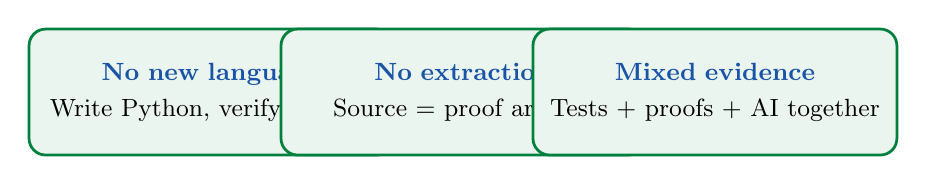
\begin{tikzpicture}[
    card/.style={rectangle, rounded corners=6pt, draw=jugeoGreen, fill=jugeoGreen!8,
                 text width=42mm, minimum height=16mm, font=\small,
                 line width=1pt, inner sep=6pt, align=center}
  ]
  \node[card] (c1) at (-3.2, 0) {\jugmark{No new language}\\[2pt]Write Python, verify Python};
  \node[card] (c2) at ( 0,    0) {\jugmark{No extraction}\\[2pt]Source = proof artifact};
  \node[card] (c3) at ( 3.2,  0) {\jugmark{Mixed evidence}\\[2pt]Tests + proofs + AI together};
\end{tikzpicture}
\end{center}
\vspace{10pt}
\begin{exampleblock}{For the first time}
  Formal verification that works \jugmark{with} Python, not against it.\\[4pt]
  Exceptions, generators, async, metaclasses --- all supported.\\[4pt]
  Your existing test suite counts as evidence from day one.
\end{exampleblock}
\end{frame}

% ---------------------------------------------------------------------------
% Slide 191: What This Means for Verification Researchers
% ---------------------------------------------------------------------------
\begin{frame}
\frametitle{What This Means for Verification Researchers}
\begin{block}{New Foundations}
  \begin{itemize}
    \item \jugmark{Sheaf-theoretic proofs} --- sections, descent, cohomology
    \item \jugmark{Multi-channel evidence} --- trust algebra over 7 levels
    \item \jugmark{Structured failures} --- obstructions classified by cohomology
  \end{itemize}
\end{block}
\vspace{6pt}
\begin{center}
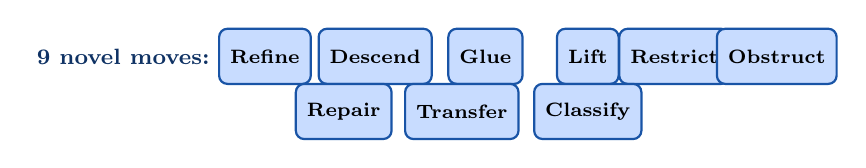
\begin{tikzpicture}[
    mv/.style={rectangle, rounded corners=3pt, draw=jugeoBlue, fill=jugeoLight,
               minimum height=7mm, font=\scriptsize\bfseries, inner xsep=4pt,
               line width=0.8pt}
  ]
  \node[font=\footnotesize\bfseries\color{jugeoDark}] at (-4.8,0) {9 novel moves:};
  \node[mv] at (-3,0)  {Refine};
  \node[mv] at (-1.6,0){Descend};
  \node[mv] at (-0.2,0){Glue};
  \node[mv] at (1.1,0) {Lift};
  \node[mv] at (2.2,0) {Restrict};
  \node[mv] at (3.5,0) {Obstruct};
  \node[mv] at (-2.0,-0.7) {Repair};
  \node[mv] at (-0.5,-0.7) {Transfer};
  \node[mv] at (1.1,-0.7)  {Classify};
\end{tikzpicture}
\end{center}
\vspace{4pt}
{\small Proof failures become \jugmark{mathematical objects} you can analyze, not just error messages.}
\end{frame}

% ---------------------------------------------------------------------------
% Slide 192: What This Means for AI and Code
% ---------------------------------------------------------------------------
\begin{frame}
\frametitle{What This Means for AI and Code}
\begin{center}
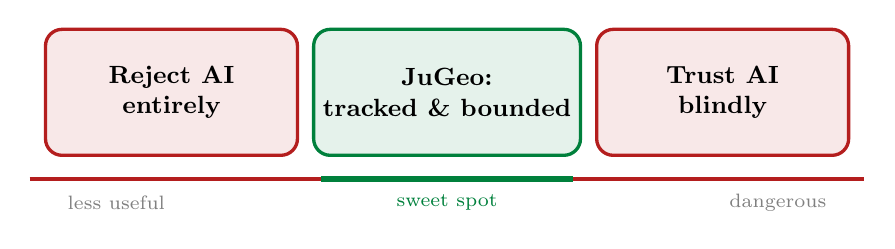
\begin{tikzpicture}[
    zone/.style={rectangle, rounded corners=6pt,
                 minimum width=32mm, minimum height=16mm, font=\small\bfseries,
                 line width=1.2pt, align=center}
  ]
  \node[zone, draw=jugeoRed, fill=jugeoRed!10]     (rej) at (-3.5,0) {Reject AI\\entirely};
  \node[zone, draw=jugeoGreen, fill=jugeoGreen!10] (jug) at ( 0,  0) {JuGeo:\\tracked \& bounded};
  \node[zone, draw=jugeoRed, fill=jugeoRed!10]     (tru) at ( 3.5,0) {Trust AI\\blindly};

  \draw[jugeoRed, line width=1.5pt]   (-5.3,-1.1) -- (5.3,-1.1);
  \draw[jugeoGreen, line width=2pt]   (-1.6,-1.1) -- (1.6,-1.1);
  \node[font=\scriptsize\color{gray}] at (-4.2,-1.4) {less useful};
  \node[font=\scriptsize\color{gray}] at ( 4.2,-1.4) {dangerous};
  \node[font=\scriptsize\color{jugeoGreen}] at (0,-1.4) {sweet spot};
\end{tikzpicture}
\end{center}
\vspace{6pt}
\begin{itemize}
  \item AI (Copilot) is a \jugmark{first-class evidence channel}
  \item Trust ceiling: AI evidence cannot exceed level 4 without corroboration
  \item Every AI-sourced claim is \jugmark{tracked, audited, bounded}
\end{itemize}
\end{frame}

% ---------------------------------------------------------------------------
% Slide 193: Future Directions — Language Support
% ---------------------------------------------------------------------------
\begin{frame}
\frametitle{Future: Beyond Python}
\begin{center}
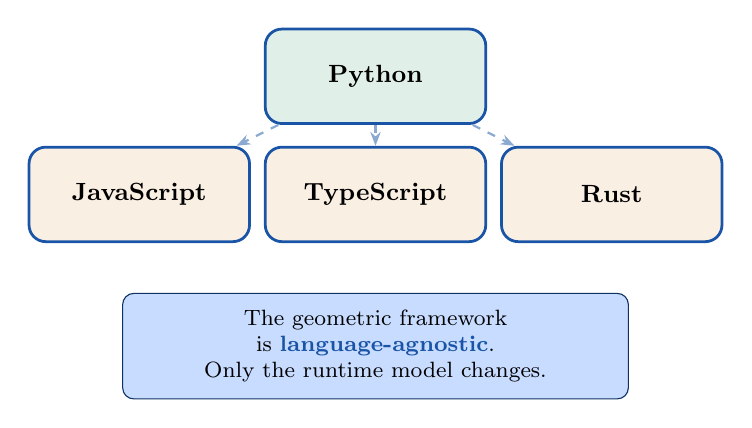
\begin{tikzpicture}[
    lang/.style={rectangle, rounded corners=6pt, draw=jugeoBlue,
                 minimum width=28mm, minimum height=12mm, font=\small\bfseries,
                 line width=1pt},
    arr/.style={-{Stealth[length=5pt]}, jugeoBlue!50, line width=0.8pt, dashed}
  ]
  \node[lang, fill=jugeoGreen!12]  (py) at (0, 1.5) {Python};
  \node[lang, fill=jugeoOrange!12] (js) at (-3,0)   {JavaScript};
  \node[lang, fill=jugeoOrange!12] (ts) at ( 0,0)   {TypeScript};
  \node[lang, fill=jugeoOrange!12] (rs) at ( 3,0)   {Rust};

  \draw[arr] (py)--(js);
  \draw[arr] (py)--(ts);
  \draw[arr] (py)--(rs);

  \node[rectangle, rounded corners=4pt, draw=jugeoDark, fill=jugeoLight,
        font=\footnotesize, inner sep=6pt, text width=60mm, align=center,
        below=18pt of ts] (note)
    {The geometric framework is \jugmark{language-agnostic}.\\
     Only the runtime model changes.};
\end{tikzpicture}
\end{center}
\vspace{4pt}
\begin{itemize}
  \item Coordinates, covers, trust, obstructions --- all transfer
  \item Each language needs its own \jugmark{runtime adapter}
  \item Community contributions welcome
\end{itemize}
\end{frame}

% ---------------------------------------------------------------------------
% Slide 194: Future Directions — Distributed Verification
% ---------------------------------------------------------------------------
\begin{frame}
\frametitle{Future: Distributed Verification}
\begin{center}
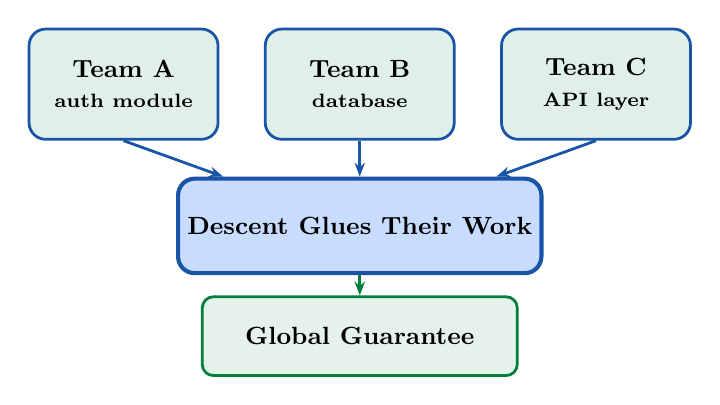
\begin{tikzpicture}[
    team/.style={rectangle, rounded corners=6pt, draw=jugeoBlue,
                 minimum width=24mm, minimum height=14mm, font=\small\bfseries,
                 line width=1pt, align=center},
    arr/.style={-{Stealth[length=5pt]}, jugeoBlue, line width=1pt}
  ]
  \node[team, fill=jugeoGreen!12]  (t1) at (-3, 1.2) {Team A\\{\scriptsize auth module}};
  \node[team, fill=jugeoGreen!12]  (t2) at ( 0, 1.2) {Team B\\{\scriptsize database}};
  \node[team, fill=jugeoGreen!12]  (t3) at ( 3, 1.2) {Team C\\{\scriptsize API layer}};

  \node[rectangle, rounded corners=6pt, draw=jugeoBlue, fill=jugeoLight,
        minimum width=40mm, minimum height=12mm, font=\small\bfseries,
        line width=1.5pt] (desc) at (0,-0.6) {Descent Glues Their Work};

  \draw[arr] (t1.south) -- (desc);
  \draw[arr] (t2.south) -- (desc);
  \draw[arr] (t3.south) -- (desc);

  \node[rectangle, rounded corners=4pt, draw=jugeoGreen, fill=jugeoGreen!10,
        minimum width=40mm, minimum height=10mm, font=\small\bfseries,
        line width=1pt] (glob) at (0,-2.0) {Global Guarantee};
  \draw[arr, jugeoGreen] (desc)--(glob);
\end{tikzpicture}
\end{center}
\vspace{4pt}
\begin{itemize}
  \item Multiple teams verify different parts of the codebase
  \item \jugmark{Trust tracks} who verified what, when, and how
  \item Descent ensures local proofs compose into global correctness
\end{itemize}
\end{frame}

% ---------------------------------------------------------------------------
% Slide 195: Future Directions — Continuous Verification
% ---------------------------------------------------------------------------
\begin{frame}
\frametitle{Future: JuGeo in CI/CD}
\begin{center}
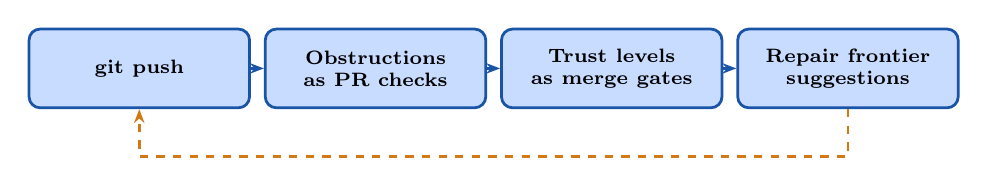
\begin{tikzpicture}[
    stage/.style={rectangle, rounded corners=4pt, draw=jugeoBlue, fill=jugeoLight,
                  minimum width=28mm, minimum height=10mm, font=\scriptsize\bfseries,
                  line width=1pt, align=center},
    arr/.style={-{Stealth[length=5pt]}, jugeoBlue, line width=1pt}
  ]
  \node[stage] (push) at (-4, 0) {git push};
  \node[stage] (obs)  at (-1, 0) {Obstructions\\as PR checks};
  \node[stage] (gate) at ( 2, 0) {Trust levels\\as merge gates};
  \node[stage] (rep)  at ( 5, 0) {Repair frontier\\suggestions};

  \draw[arr] (push)--(obs);
  \draw[arr] (obs)--(gate);
  \draw[arr] (gate)--(rep);

  % feedback loop
  \draw[arr, dashed, jugeoOrange] (rep.south) -- ++(0,-0.6) -| (push.south);
\end{tikzpicture}
\end{center}
\vspace{8pt}
\begin{center}
\begin{tabular}{@{} l l @{}}
\toprule
\textbf{CI/CD Concept} & \textbf{JuGeo Mapping} \\
\midrule
PR check        & Obstruction report \\
Merge gate      & Minimum trust level \\
Auto-suggestion & Repair frontier \\
Dashboard       & Trust heatmap over coordinates \\
\bottomrule
\end{tabular}
\end{center}
\end{frame}

% ---------------------------------------------------------------------------
% Slide 196: Getting Started
% ---------------------------------------------------------------------------
\begin{frame}[fragile]
\frametitle{Getting Started}
\begin{block}{Install and run in 30 seconds}
\begin{lstlisting}
pip install -e .
pytest test_examples/ -v
python3 test_algorithms.py
\end{lstlisting}
\end{block}
\vspace{6pt}
\begin{exampleblock}{Requirements}
  \begin{itemize}
    \item Python $\geq$ 3.10
    \item No external solvers needed for basic usage
    \item Optional: Z3 for SMT channel, Copilot for AI channel
  \end{itemize}
\end{exampleblock}
\vspace{6pt}
\begin{center}
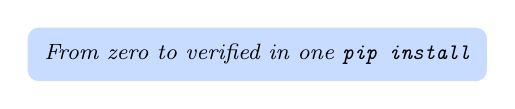
\begin{tikzpicture}
  \node[fill=jugeoLight, rounded corners, inner sep=6pt, font=\footnotesize\itshape]
    {From zero to verified in one \texttt{pip install}};
\end{tikzpicture}
\end{center}
\end{frame}

% ---------------------------------------------------------------------------
% Slide 197: Key Takeaways — 5 Things to Remember
% ---------------------------------------------------------------------------
\begin{frame}
\frametitle{Five Things to Remember}
\begin{center}
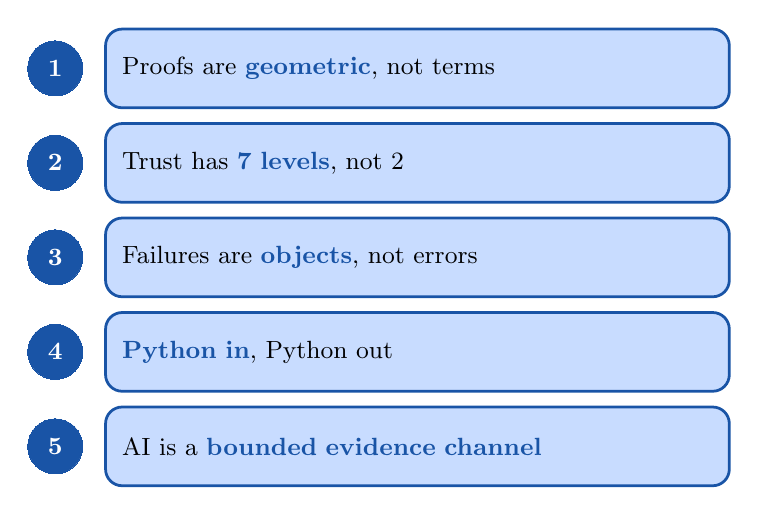
\begin{tikzpicture}[
    item/.style={rectangle, rounded corners=6pt, draw=jugeoBlue, fill=jugeoLight,
                 text width=75mm, minimum height=10mm, font=\small,
                 line width=1pt, inner sep=6pt},
    num/.style={circle, draw=jugeoBlue, fill=jugeoBlue, text=white,
                minimum size=7mm, font=\small\bfseries, line width=0pt}
  ]
  \node[item] (i1) at (0, 2.8) {Proofs are \jugmark{geometric}, not terms};
  \node[item] (i2) at (0, 1.6) {Trust has \jugmark{7 levels}, not 2};
  \node[item] (i3) at (0, 0.4) {Failures are \jugmark{objects}, not errors};
  \node[item] (i4) at (0,-0.8) {\jugmark{Python in}, Python out};
  \node[item] (i5) at (0,-2.0) {AI is a \jugmark{bounded evidence channel}};

  \node[num] at (-4.6, 2.8) {1};
  \node[num] at (-4.6, 1.6) {2};
  \node[num] at (-4.6, 0.4) {3};
  \node[num] at (-4.6,-0.8) {4};
  \node[num] at (-4.6,-2.0) {5};
\end{tikzpicture}
\end{center}
\end{frame}

% ---------------------------------------------------------------------------
% Slide 198: The JuGeo Motto
% ---------------------------------------------------------------------------
\begin{frame}
\frametitle{}
\vfill
\begin{center}
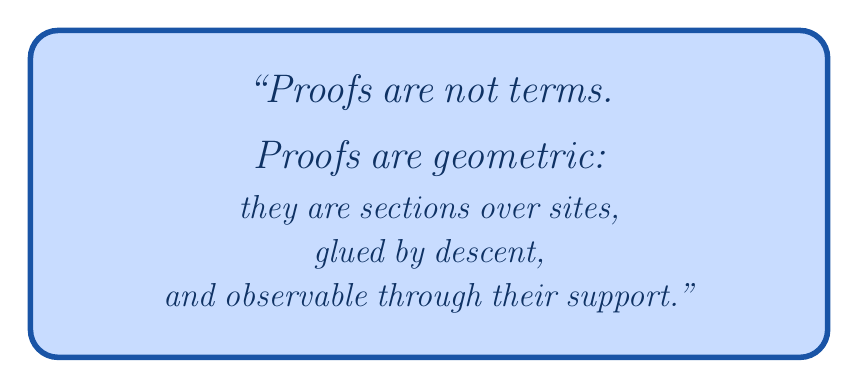
\begin{tikzpicture}
  \node[rectangle, rounded corners=10pt, draw=jugeoBlue, fill=jugeoLight,
        line width=2pt, inner sep=16pt, text width=90mm, align=center]
    {{\Large\color{jugeoDark}\itshape
      ``Proofs are not terms.}\\[10pt]
     {\Large\color{jugeoDark}\itshape
      Proofs are geometric:}\\[6pt]
     {\large\color{jugeoDark}\itshape
      they are sections over sites,}\\[4pt]
     {\large\color{jugeoDark}\itshape
      glued by descent,}\\[4pt]
     {\large\color{jugeoDark}\itshape
      and observable through their support.''}};
\end{tikzpicture}
\end{center}
\vfill
\end{frame}

% ---------------------------------------------------------------------------
% Slide 199: Thank You
% ---------------------------------------------------------------------------
\begin{frame}
\frametitle{Thank You}
\vfill
\begin{center}
  {\LARGE\color{jugeoBlue}\textbf{Thank you!}}\\[20pt]
  
\begin{tikzpicture}
    \draw[jugeoBlue, line width=1.5pt] (-2.5,0) -- (2.5,0);
  \end{tikzpicture}\\[16pt]
  {\large\color{jugeoDark} JuGeo --- Judgment Geometry for Python}\\[12pt]
  {\small\color{gray}
    \texttt{github.com/jugeo/jugeo}\\[4pt]
    \texttt{contact@jugeo.dev}\\[4pt]
    Documentation: \texttt{jugeo.readthedocs.io}}
\end{center}
\vfill
\end{frame}

% ---------------------------------------------------------------------------
% Slide 200: Questions?
% ---------------------------------------------------------------------------
\begin{frame}
\frametitle{Questions?}
\vfill
\begin{center}
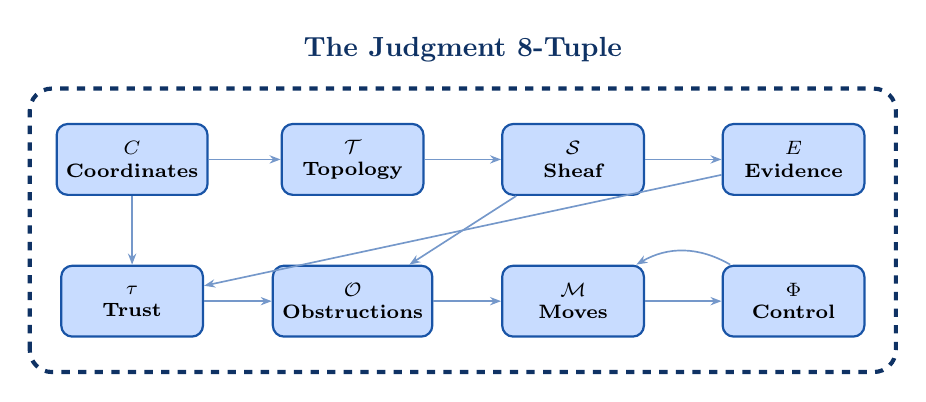
\begin{tikzpicture}[
    comp/.style={rectangle, rounded corners=4pt, draw=jugeoBlue, fill=jugeoLight,
                 minimum width=18mm, minimum height=9mm, font=\scriptsize\bfseries,
                 line width=0.8pt, align=center},
    lbl/.style={font=\tiny\color{jugeoDark}, align=center},
    arr/.style={-{Stealth[length=4pt]}, jugeoBlue!60, line width=0.6pt}
  ]
  % The 8-tuple diagram
  \node[font=\normalsize\bfseries\color{jugeoDark}] at (0,3.2) {The Judgment 8-Tuple};

  \node[comp] (C) at (-4.2, 1.8) {$C$\\Coordinates};
  \node[comp] (T) at (-1.4, 1.8) {$\mathcal{T}$\\Topology};
  \node[comp] (S) at ( 1.4, 1.8) {$\mathcal{S}$\\Sheaf};
  \node[comp] (E) at ( 4.2, 1.8) {$E$\\Evidence};

  \node[comp] (tau) at (-4.2, 0) {$\tau$\\Trust};
  \node[comp] (O)   at (-1.4, 0) {$\mathcal{O}$\\Obstructions};
  \node[comp] (M)   at ( 1.4, 0) {$\mathcal{M}$\\Moves};
  \node[comp] (Phi) at ( 4.2, 0) {$\Phi$\\Control};

  % Connections
  \draw[arr] (C)--(T);
  \draw[arr] (T)--(S);
  \draw[arr] (S)--(E);
  \draw[arr] (C)--(tau);
  \draw[arr] (E)--(tau);
  \draw[arr] (tau)--(O);
  \draw[arr] (O)--(M);
  \draw[arr] (M)--(Phi);
  \draw[arr] (S)--(O);
  \draw[arr] (Phi) to[bend right=30] (M);

  % Surrounding box
  \draw[jugeoDark, rounded corners=8pt, line width=1.5pt, dashed]
    (-5.5,-0.9) rectangle (5.5,2.7);
\end{tikzpicture}
\end{center}
\vspace{6pt}
\begin{center}
  {\Large\color{jugeoBlue}\textbf{?}}\\[4pt]
  {\small\color{jugeoDark} Geometry in, geometry out --- all the way down.}
\end{center}
\vfill
\end{frame}

\end{document}
